\documentclass[aspectratio=169]{beamer}
\usetheme{default}
\usetikzlibrary{arrows.meta,positioning}

\title{hatex}
\subtitle{\LaTeX{} articles and slides, rendered in the browser}
\author{Mejistus}
\date{September 2026}

\begin{document}

\begin{frame}
  \titlepage
\end{frame}

\begin{frame}{Outline}
  \tableofcontents
\end{frame}

\section{Why hatex}
\begin{frame}{hatex = HTML + \LaTeX}
  \begin{itemize}
    \item<1-> Notes and papers are written in \LaTeX.
    \item<2-> The web wants HTML: links, search, any screen size.
    \item<3-> hatex turns one into the other, in the browser, with no TeX installation and no build step.
  \end{itemize}
  \begin{exampleblock}{This deck}
    One \texttt{.tex} file with \verb|\documentclass{beamer}|, fetched and rendered by hatex.
  \end{exampleblock}
\end{frame}

\section{How it works}
\begin{frame}{From source to page}
  \begin{center}
    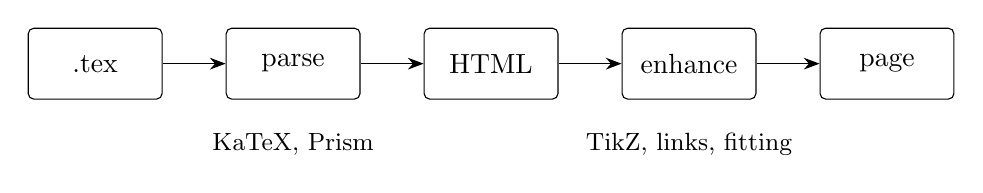
\begin{tikzpicture}[node distance=8mm, >={Stealth[length=2mm]},
        box/.style={draw, rounded corners=2pt, minimum height=9mm, minimum width=17mm, align=center}]
      \node[box] (tex) {.tex};
      \node[box, right=of tex] (parse) {parse};
      \node[box, right=of parse] (html) {HTML};
      \node[box, right=of html] (enh) {enhance};
      \node[box, right=of enh] (page) {page};
      \draw[->] (tex) -- (parse);
      \draw[->] (parse) -- (html);
      \draw[->] (html) -- (enh);
      \draw[->] (enh) -- (page);
      \node[below=3mm of parse, font=\small] {KaTeX, Prism};
      \node[below=3mm of enh, font=\small] {TikZ, links, fitting};
    \end{tikzpicture}
  \end{center}
  \texttt{parse} needs no DOM, so it also runs in Node at build time.
  \texttt{enhance} does what only a live page can: compiling TikZ, scrolling to references, fitting wide tables.
\end{frame}

\begin{frame}[fragile]{Using it}
\begin{lstlisting}[language=html]
<link rel="stylesheet" href="katex.min.css">
<script src="katex.min.js"></script>
<script src="hatex.js"></script>

<div id="deck"></div>
<script>
  fetch('slides.tex')
    .then(r => r.text())
    .then(tex => HaTeX.render('#deck', tex));
</script>
\end{lstlisting}
\end{frame}

\section{What it renders}
\begin{frame}[t]{Maths}
  \begin{columns}[T]
    \begin{column}{0.5\textwidth}
      Numbered display maths:
      \begin{equation}\label{eq:gauss}
        \int_{-\infty}^{\infty} e^{-x^2}\,\mathrm{d}x = \sqrt{\pi}
      \end{equation}
      and inline maths, $\nabla_x \log q_t(x) = -\epsilon / \sqrt{1-\bar\alpha_t}$.
    \end{column}
    \begin{column}{0.5\textwidth}
      \begin{block}{Tweedie's formula}
        $\mathbb{E}[x_0 \mid x_t] = \dfrac{x_t + (1-\bar\alpha_t)\,\nabla \log q_t(x_t)}{\sqrt{\bar\alpha_t}}$
      \end{block}
      \begin{alertblock}{Cross-references}
        \eqref{eq:gauss} links back to its slide.
      \end{alertblock}
    \end{column}
  \end{columns}
\end{frame}

\begin{frame}{Tables}
  \begin{center}
    \begin{tabular}{lcc}
      \toprule
      & Articles & Slides \\
      \midrule
      Maths, tables, figures, code & yes & yes \\
      TikZ and pgfplots & yes & yes \\
      Two columns, \texttt{multicols} & yes & --- \\
      Blocks and columns & yes & yes \\
      Overlays (\verb|\pause|, \verb|<2->|) & --- & all steps at once \\
      \bottomrule
    \end{tabular}
  \end{center}
\end{frame}

\begin{frame}{Blocks}
  \begin{block}{block}
    For definitions and results.
  \end{block}
  \begin{alertblock}{alertblock}
    For things to watch out for, and \alert{alerted} words.
  \end{alertblock}
  \begin{exampleblock}{exampleblock}
    For examples.
  \end{exampleblock}
\end{frame}

\section{Presenting}
\begin{frame}{Presenting}
  \begin{itemize}
    \item \textbf{Present}, or a double-click on a slide, goes full screen.
    \item Right arrow, Space or a click: next. Left arrow: back. Esc: leave.
    \item Slides are laid out at a fixed size and scaled to the screen, so they look the same everywhere.
    \item Content taller than a slide is shrunk to fit.
  \end{itemize}
\end{frame}

\begin{frame}[plain]
  \begin{center}
    {\Huge Thank you}

    \url{https://mejistus.github.io/hatex/}
  \end{center}
\end{frame}

\end{document}
